\subsection{Архитектура решения}
\paragraph{}

Архитектура предлагаемого решение приведена на рисунке \ref{fig:arch}.
\begin{figure}[h!]
\centering
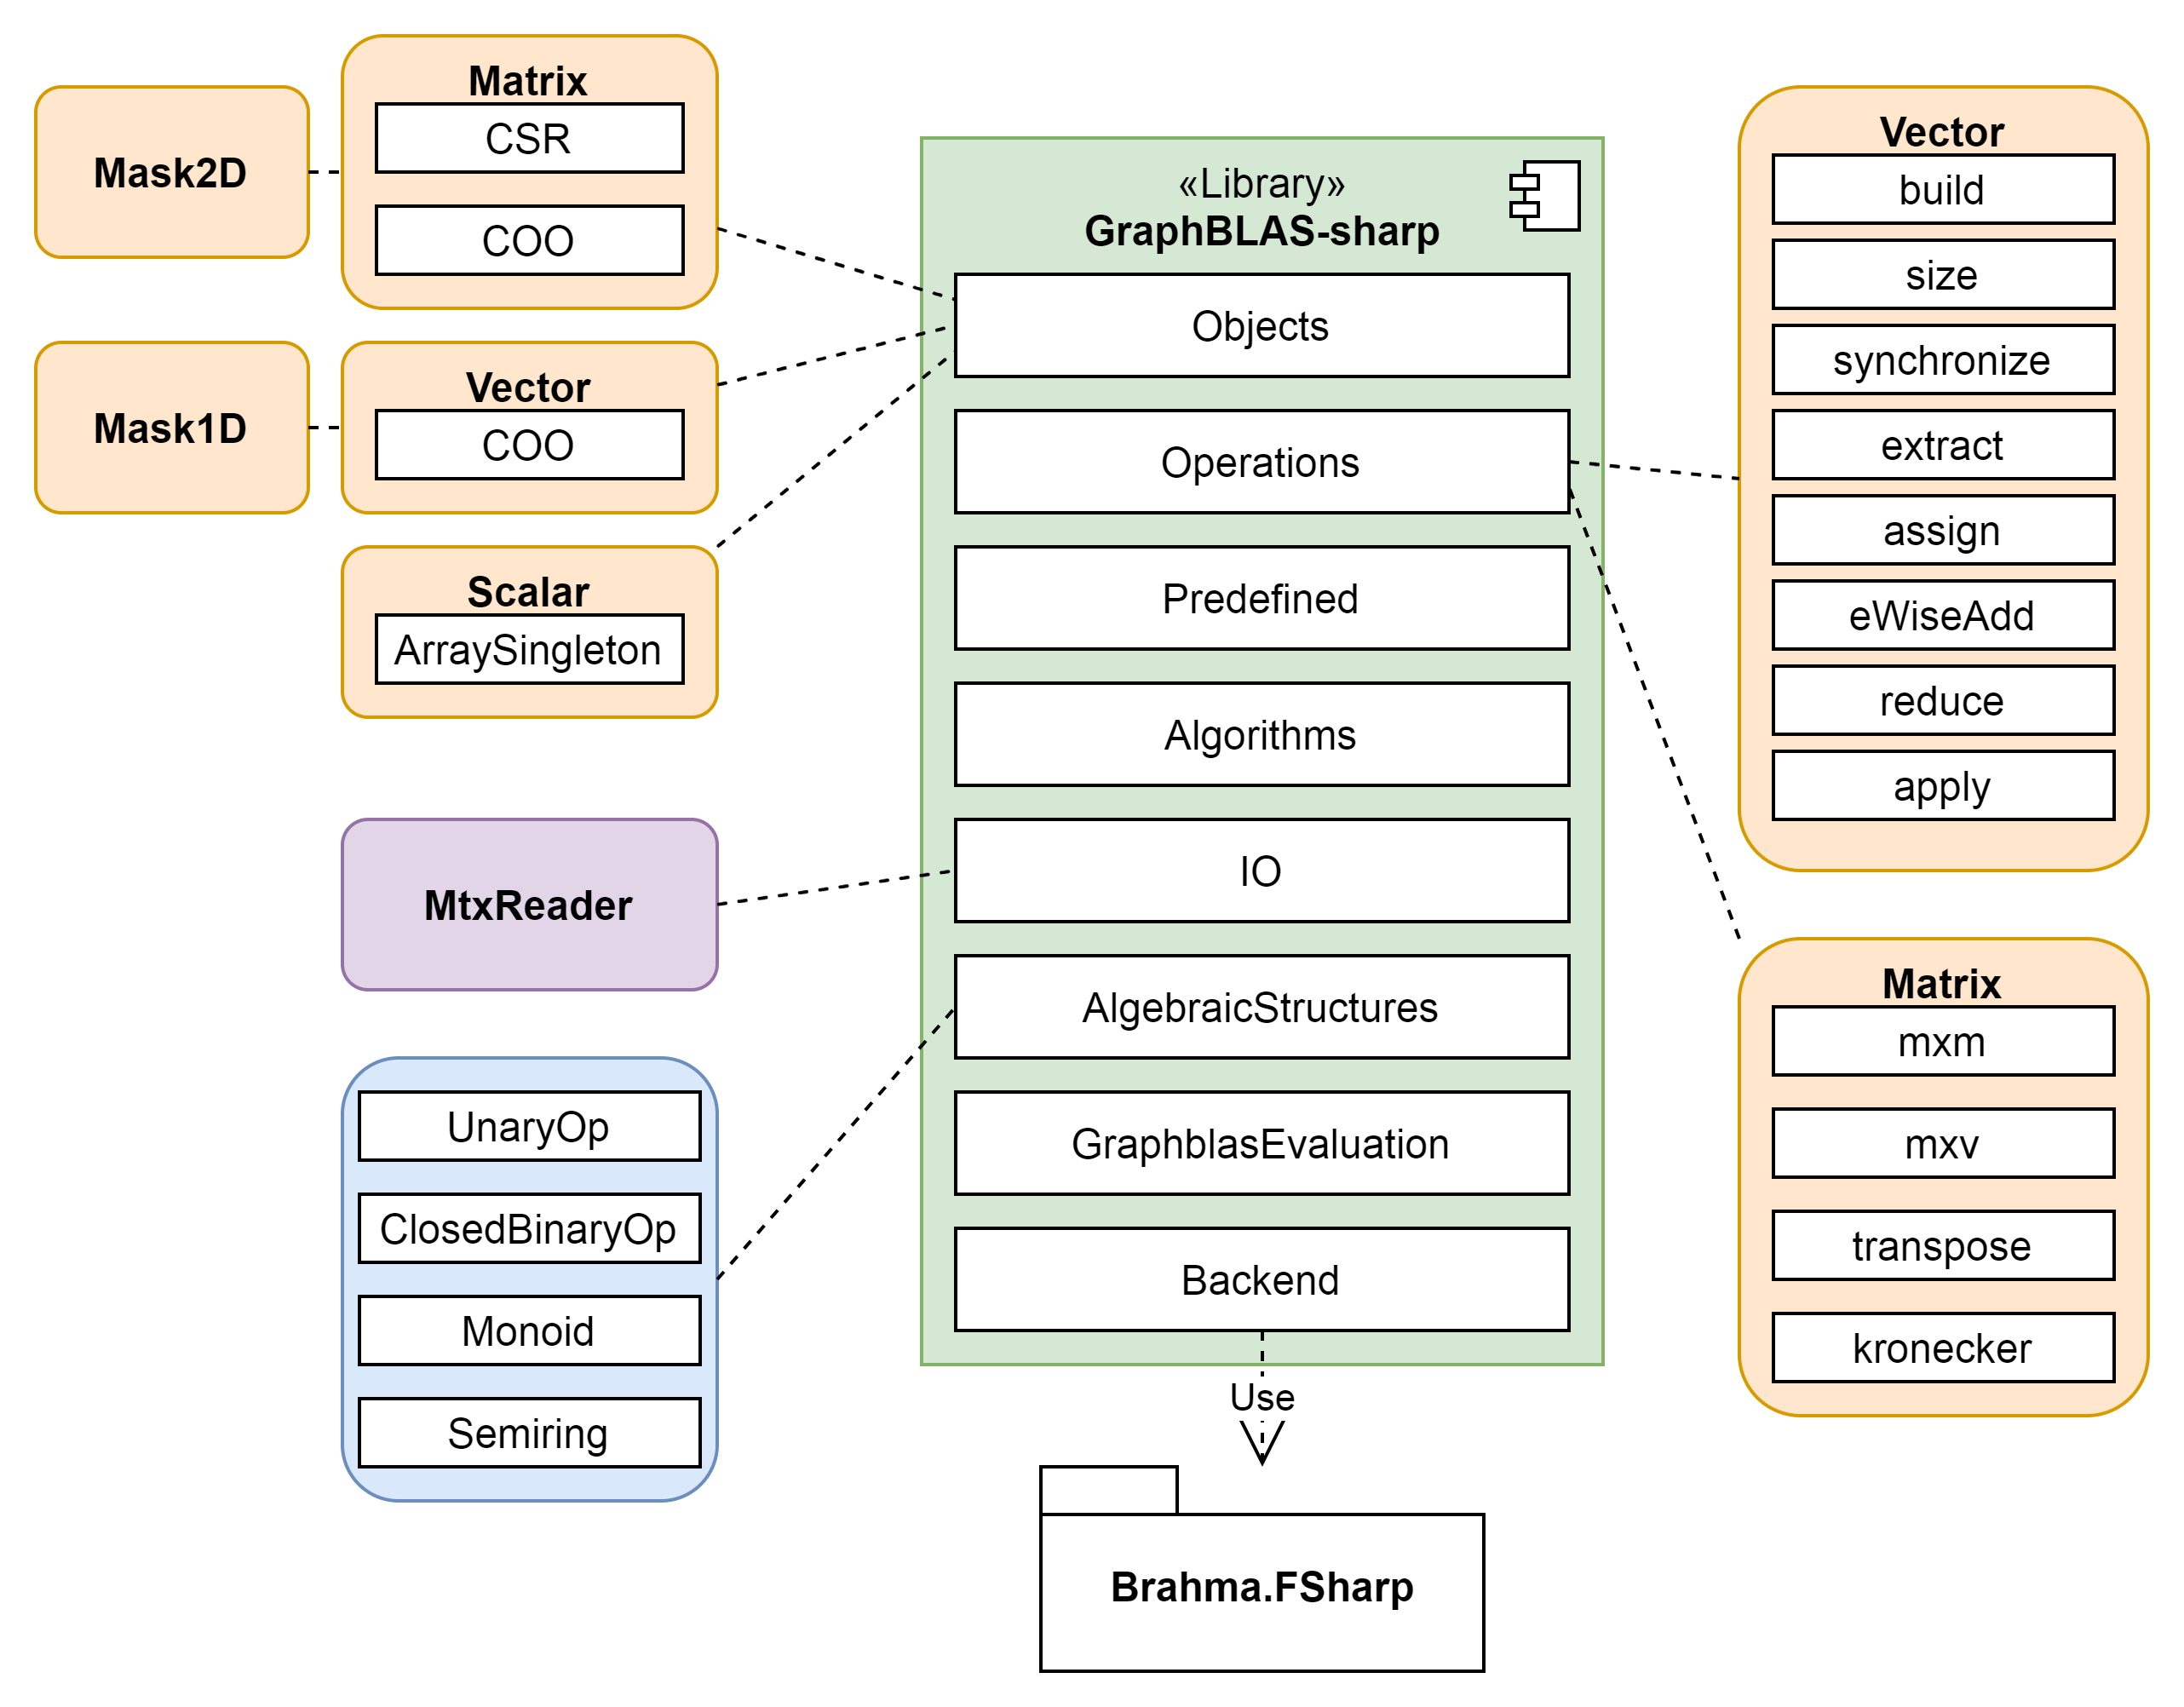
\includegraphics[scale=0.5]{pictures/dia3.png}
\caption{Архитектура предлагаемой библиотеки GraphBLAS-sharp}
\label{fig:arch}
\end{figure}

В рамках данной работы были реализованы компоненты библиотеки GraphBLAS-sharp, описанные ниже.
\begin{itemize}
    \item \textbf{Модули коллекций Matrix и Vector}. Модули содержат абстрактные классы для представления матрицы и вектора, реализованные в виде размеченного объединения, а также конкретные форматы их хранения.
    \item \textbf{Модули операций Matrix и Vector}. Модули содержат определение операций стандарта GraphBLAS для работы с абстрактными коллекциями.
    \item \textbf{Модуль AlgebraicStructures}. Модуль содержит реализацию не\-ко\-то\-рых алгебраических структур, таких как моноид и полукольцо.
    \item \textbf{Модуль Predefined}. Модуль содержит реализацию представителей классов алгебраических структур для встроенных типов данных. Так, например, в модуле реализованно стандартное булево полукольцо, стандартное арифметическое полукольцо над встроенными типами данных, а также тропическое полукольцо.
    \item \textbf{Модуль GraphblasEvaluation}. Модуль содержит вычислительное выражение GraphblasEvaluation. Оно выполняет 2 функции --- во-первых, являясь по своей сути монадой Reader, позволяет выставлять глобальные и локальные параметры вычисления, а во-вторых, оно скрывает использование интерфейса для работы с OpenCL, который предоставляет библиотека Brahma.Fsharp.
    \item \textbf{Модуль MtxReader}. Модуль предназначен для импорта матриц из файлов в формате \textit{mtx}.
    \item \textbf{Модуль Algorithms}. Модуль содержит небольшой набор классических алгоритмов на графах. В нем реализованы следующие алгоритмы: 
    \begin{itemize}
        \item алгоритм поиска в ширину из единственной вершины
        \item алгоритм поиска кратчайшего пути из единственной вершины
        \item алгоритм подсчета числа треугольников в графе
        \item алгоритм вычисления меры центральности вершины
    \end{itemize}
    \item \textbf{Модуль Backend}. Модуль содержит реализацию соответствующих операций для конкретных форматов хранения матрицы и вектора. В рамках данной работы были реализованны следующие операции:
    \begin{itemize}
        \item умножение матрицы в CSR формате на разреженный вектор
        \item транспонирование матрицы в CSR формате
        \item создание разреженного вектора из списка элементов
    \end{itemize}
\end{itemize}

\subsection{Реализация коллекций}
\paragraph{}
Особенностью стандарта GraphBLAS является то, что описываемые в нем объекты абстрактны --- за реализацию внутреннего хранения объектов ответственен разработчик решения. 

В качестве форматов хранения матрицы используются 2 формата --- CSR и COO.
Матрицы, которые выражают графы, обычно сильно разреженны, поэтому использовать плотную матрицу в качестве внутренней реализации нецелесообразно.
CSR формат, по сравнению, например, с диагональным (DIA) или ELLPACK (ELL) форматом, лучше подходит для хранения произвольных разреженных матриц, так как не требует от матрицы соответствия определенному паттерну для эффективного хранения. По сравнению с COO он занимает $2 \cdot nnz + n + 1$ вместо $3\cdot nnz$ памяти (здесь и далее $nnz$ --- число ненулевых элементов матрицы, $n$ --- число строк матрицы, $m$ --- число столбцов) и предоставляет доступ к произвольной строке за $O(1)$, что является существенным преимущество при реализации параллельных алгоритмов. В то же время для хранения сверхразреженных матриц, у которых $nnz > (m\cdot(n-1)-1)/2$ лучше подходит формат COO.

\subsection{Реализация операций}
\subsubsection{Умножение матрицы в CSR формате на разреженный вектор}
\paragraph{}
Для реализации операции умножения матрицы на вектор были рассмотрены несколько алгоритмов. В статье за авторством W. Liu and B. Vinter\cite{esc} приводится алгоритм умножения разреженных матриц в CSR формате. Ключевой операцией в алгоритмах такого рода является операция слияния строк промежуточной матрицы. Так как все строки имеют разное число ненулевых элементов, то для данной операции особо важно выбрать эффективный метод балансирования нагрузки. В данной статье предлагается разделить все строки промежуточной матрицы на 38 групп в зависимости числа ненулевых элементов в них и для каждой группы использовать один из четырех алгоритмов слияния. Однако, как показывает последние работы в данной области\cite{hash}, существуют более производительные и простые в решения. Так, статья за авторством Y. Nagasaka и др.\cite{hash}, которая также описывает алгоритм умножения разреженных матриц в CSR формате, предлагает для слияния строк использовать хеш-таблицу. По словам автора, этот алгоритм выигрывает у предыдущего и по времени работы, и по количеству потребляемой памяти. Однако для обновления данных в хеш-таблице алгоритм использует атомарные операции, а атомарные операции над произвольными типами на данный момент не поддерживаются библиотекой Brahma.FSharp, поэтому реализовать данный алгоритм оказалось невозможно. Алгоритм, описывающий умножение матрицы в CSR формате на разреженный вектор, за авторством Y. Tao и др.\cite{atomic} также предполагает использование атомарных операций, что делает невозможным его реализацию. Другой метод авторов Yang, C., Wang, Y., и Owens, J. D\cite{mxv_bfs} описывает умножения матрицы в CSR формате на разреженный вектор в контексте применения его в алгоритмах, подобных алгоритму поиска в ширину, а при оценке эффективности работы использует допущение о том, что вектор имеет небольшое число ненулевых элементов. Несмотря на то, что именно этот алгоритм реализован в аналогичной библиотеке GraphBLAST, было решено отказаться от него в пользу альтернативного варианта. В предлагаемой работе был реализован следующий алгоритм.
\begin{enumerate}
    \item Каждая строка матрицы умножается на разреженный вектор.
    \begin{itemize}
        \item Каждая строка обрабатывается 1 рабочей группой.
        \item Каждый поток в рабочей группе обрабатывает 1 элемент левого вектора с шагом, равным размеру рабочей группы.
        \item Значение с нужным индексом в правом векторе ищется бинарным поиском.
    \end{itemize}
    \item Полученный вектор промежуточных значений фильтруется от нулевых элементов с использованием префиксной суммы.
\end{enumerate}

\subsubsection{Транспонирование матрицы в CSR формате}
\paragraph{}
Для транспонирования матрицы в CSR формате был реализован наивный алгоритм, предполагающий конвертацию матрицы в формат COO.
\begin{enumerate}
    \item Матрица в CSR формате конвертируется в формат COO.
    \item Индексы элементов сортируются битонической сортировкой так, чтобы соответствовать транспонированной матрице.
    \item Матрица в COO формате конвертируется обратно в формат CSR.
\end{enumerate}

\subsection{Тестирование и непрерывная интеграция}
\paragraph{}
Использование высокоуровневого языка для реализации стандарта GraphBLAS, в том числе, облегчает тестирование. В GraphBLAS внутреннее поведение операции зависит от объектов управления и от того, как именно реализованы абстрактные объекты коллекций, причем с ростом числа используемых реализаций число вариантов операции, которые нужно тестировать, растет экспоненциально. В реализациях на С++, в которых для тестирования применялся Boost Test Framework, отдельно тестируется каждый вариант и, как правило, только на одном типе данных. 

В данной работе для тестирования используется библиотека Expecto\footnote{Репозиторий библиотеки Expecto: \url{https://github.com/haf/expecto}. Дата посещения: 01.06.2021}. За счет интеграции с библиотекой FsCheck\footnote{Репозиторий библиотеки FsCheck: \url{https://github.com/fscheck/FsCheck}. Дата посещения: 01.06.2021}, она поддерживает property-based тестирование, что позволяет автоматически генерировать наборы данных для тестов. Кроме того, она позволяет писать комбинаторные параметрические тесты, благодаря чему можно легко проверить все возможные варианты операции.

Возможность исполнения на CPU программ, которые используют OpenCL, позволила легко настроить тестирование библиотеки в сервисах непрерывной интеграции, таких как AppVeyor и GitHub Actions. 